\documentclass[10pt]{article}

\usepackage[ngerman]{babel}
%%% Für PDFLatex
%\usepackage[utf8]{inputenc}
%\usepackage[T1]{fontenc}
%%% Für XeLaTeX
\usepackage{fontspec}
\setmainfont{DejaVu Sans}
%%%
\usepackage{graphicx}
\usepackage[
	a4paper,
	top=1cm,
	bottom=2cm,
	right=2cm,
	left=2.5cm]{geometry}
\usepackage{booktabs}
\usepackage{tabularx}

\begin{document}
\section{Inbetriebnahme}
\begin{enumerate}
\item Überprüfen Sie, dass das LCD-Display eingesteckt ist.
\item Überprüfen Sie, dass der Jumper J9 (Temperatursensor) den Sensor mit dem Pin PB2 verbindet.
\item Überprüfen Sie, dass der Jumper J12 (simuliertes Hygrometer) den Sensor mit dem Pin PA2 verbindet.
\item Schließen Sie das Board an die Stromversorgung an.
\item Wenn benötigt stellen Sie mit dem USB-Kabel eine Verbindung zu einem Computer her.
\item Schalten Sie das Board mit dem Schalter POWER SUPPLY ein.
\end{enumerate}
\section{Bedienung}
\begin{enumerate}
\item Bei Programmstart muss die aktuelle Uhrzeit eingestellt werden. Durch Blinken wird angezeigt, ob die Stunden oder die Minuten eingestellt werden.
	\begin{enumerate}
	\item Mit Hilfe der Pfeiltasten \texttt{Hoch} und \texttt{Runter} können die Stunden bzw. Minuten erhöht oder verringert werden.
	\item Die Einstellung wird jeweils mit \texttt{Enter} bestätigt.
	\end{enumerate}
\item Nach Einstellung der Uhrzeit befindet sich das Programm im Anzeigemodus und zeigt standardmäßig die Uhrzeit an.
\item Durch drücken der Taste \texttt{Enter} gelangt man in das Einstellungsmenü
	\begin{enumerate}
	\item Mit Hilfe der Pfeiltasten \texttt{Hoch} und \texttt{Runter} kann zwischen den Menüpunkten \textit{Uhrzeit einstellen}, sowie \textit{Displaymodus einstellen} gewählt werden. Die Auswahl wird jeweils mit der Taste \texttt{Enter} bestätigt.
	\item Die Einstellung der Uhrzeit erfolgt analog zu Punkt 1.
	\item Die Einstellung des Displaymodus erfolgt mit Hilfe der Pfeiltasten \texttt{Hoch} und \texttt{Runter} und wird mit der Taste \texttt{Enter} bestätigt. Anschließend befindet sich das Programm wieder im Anzeigemodus und stellt den gewählten Displaymodus dar.
	\end{enumerate}
\end{enumerate}
\begin{figure}[h]
\centering
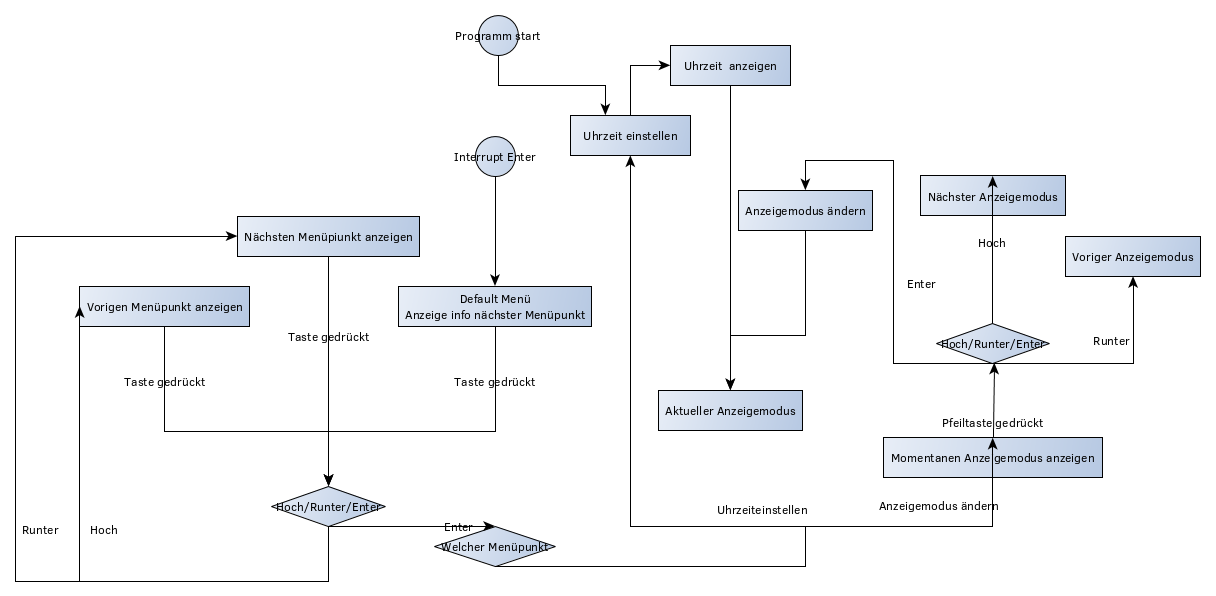
\includegraphics[width=\textwidth]{img/Programmablauf.png}
\caption{Die Menüführung graphisch dargestellt}
\end{figure}
\section{Konfiguration}
Das Programm lässt sich in der Datei Global.h konfigurieren. Hier lässt sich einstellen an welchen Pins die Sensoren und Taster angeschlossen sind. Außerdem kann angegeben werden über welchen Port das LDC-Display angesteuert wird.
\end{document}